\chapter{Implementazione}
\section{Struttura del progetto}
La struttura del progetto, organizzato in package, è la seguente:
\begin{itemize}
    \item \textbf{Actions}: le azioni della simulazione.
    \item \textbf{GlobalActions}: le azioni globali della simulazione.
    \item \textbf{Layer}: il layer personalizzato della simulazione.
    \item \textbf{NodeProperty}: le proprietà dei nodi della simulazione.
\end{itemize}

\section{Layer}
Il \textit{PheromoneLayer}, layer personalizzato della simulazione, è stato implementato come una interfaccia che estende \texttt{Layer}, 
interfaccia propria di Alchemist.  I metodi che sono definiti sono:
\begin{itemize}
    \item \texttt{void evaporate(P position, Double value)}: metodo che permette di far evaporare il feromone. 
    Richiede in input la posizione e il valore del feromone.
    \item \texttt{void deposit(P position, Double value)}: metodo che permette di far diffondere il feromone.
     Richiede in input la posizione e il valore del feromone.
    \item \texttt{Rectangle getLayerBounds()}: metodo che restituisce un oggetto di tipo \texttt{Rectangle}.
\end{itemize}

\begin{figure}[ht]
    \centering
    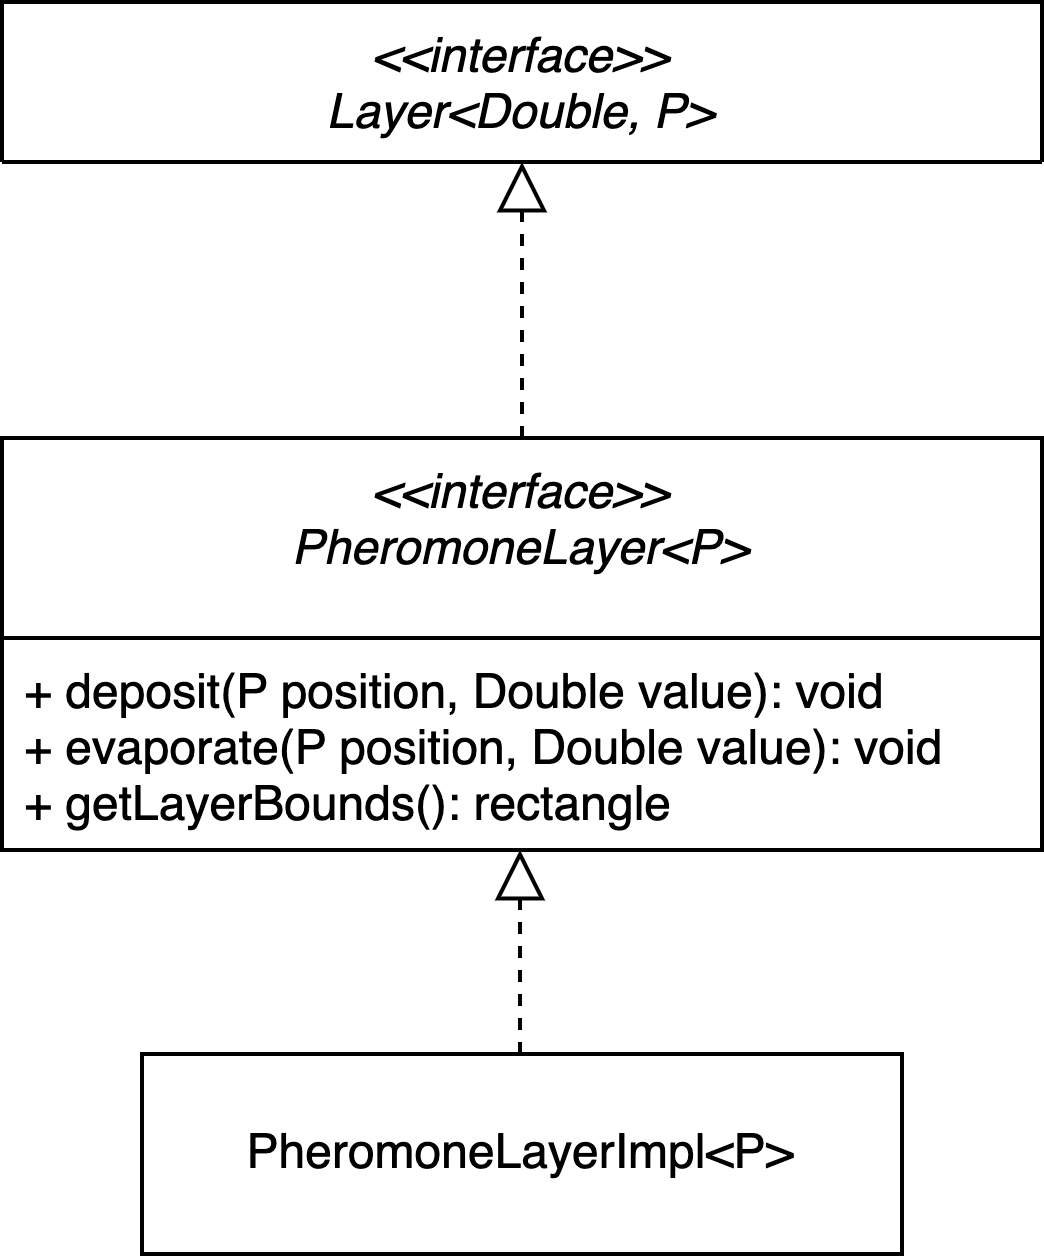
\includegraphics[width=.5\linewidth]{figures/pheromoneLayer.png}
    \caption{Struttura PheromoneLayer}\label{fig:phLayer}
\end{figure}

